%
% ---------------------------------------------------
%
% Trabajo Fin de Grado:
% Author: Víctor Hernández Pérez 
% Correo: alu0100697032@ull.edu.es
% Capítulo: Desarrollo
%
% ----------------------------------------------------
%
\chapter{Desarrollo} \label{chap:Desarrollo}  

En este capítulo se describirá, por un lado, la implementación de las 
Actividades y Clases más relevantes de la aplicación móvil y, por otro lado, los 
modelos y vistas desarrollados en Django.

\section{Django Allauth}

Django Allauth \cite{URL::allauth} es una aplicación en Django
que permite autenticación local (usuario/contraseña) y autenticación social 
(Facebook, Google y muchos otros más). La instalación se hace mediante el 
sistema de gestión de paquetes de Python (pip), 
una vez instalado se ha de configurar apropiadamente el fichero settings de la 
aplicación Django e indicar qué proveedores (para la autenticación social) son 
necesarios. 

\lstinputlisting[language=python, caption={Archivo de configuración}, label={code:settings}]
{listings/settings.py}

Por último, configurar correctamente las urls y migrar las bases de 
datos para que se creen las tablas que almacenarán la información del usuario
correspondiente al proveedor. 

\lstinputlisting[language=python, caption={URLs de la aplicación}, label={code:urls}]
{listings/urls.py} %% LISTING

\subsection{La vista \textit{login\_by\_token} para Facebook}
La propia aplicación de Allauth tiene configurada una vista que permite autenticar al usuario a través de un \textit{access token} de Facebook. Esta vista comprueba que el token recibido sea válido y en caso afirmativo pide a Facebook un token de larga duración. Dado que el token que se genera en el dispositivo móvil ya es de larga duracion, se ha reescrito la vista para que simplemente se compruebe la validez del token y autentique al usuario en la base de datos.  
\newline
\lstinputlisting[language=python, caption={Obtiene la información del token de Facebook}, label={code:check}]
{listings/checkToken.py} %% LISTING

\lstinputlisting[language=python, caption={Vista \textit{login\_by\_token} para Facebook}, label={code:loginToken}]
{listings/loginByToken.py} %% LISTING

\subsection{La vista \textit{login\_by\_token} para Google}

Para el caso de Google ha sido necesario implementar una vista similar a la de Facebook, mencionada anteriormente, para que de la misma manera, a través de un \textit{access token} de Google se pueda autenticar al usuario. 
\newline

La manera más fácil de validar el token es haciendo una petición a la url \textit{https://www.googleapis.com/oauth2/v3/tokeninfo?id\_token=xxxx} dónde \textit{xxxx} es el token del usuario.
\newline
\lstinputlisting[language=python, caption={Vista \textit{login\_by\_token} para Google}, label={code:check}]
{listings/googleLoginByToken.py} %% LISTING

Si el token está correctamente firmado y los campos \textit{iss} y \textit{exp} tienen los valores esperados, se obtendrá una respuesta HTTP 200, donde el cuerpo será un JSON como el siguiente: 

\lstinputlisting[language=java, caption={Respuesta JSON correcta}, label={code:loginToken}]
{listings/tokenInfo.json} %% LISTING

Una vez obtenida la respuesta, hay que comprobar que el campo \textit{aud} contiene el ID del cliente de la aplicación. Si es así el token es válido y se puede dar paso a la autenticación al usuario.
\newline

\lstinputlisting[language=python, caption={Obtiene la información del token de Google}, label={code:loginToken}]
{listings/googleCheckToken.py} %% LISTING

\section{Servicio de reserva de pistas}

El objetivo de que el usuario se autentique es que pueda tener acceso a algún tipo de servicio. Se ha supuesto el caso de un sistema de reserva de pistas que permite al usuario elegir una pista y una fecha y realizar la reserva de la misma.

\subsection{Modelos}
Se han creado los modelos Pista y Reserva. El modelo Pista cuenta con los campos \textit{nombre} y \textit{tipoPista}. El modelo Reserva tiene los campos \textit{pista}, \textit{usuario} y \textit{fecha}. En el modelo Reserva se indica que no pueden haber dos reservas en la base de datos de la misma pista en la misma fecha.
\newline 

\lstinputlisting[language=python, caption={Modelo Reserva}, label={code:models}]
{listings/modeloReserva.py} %% LISTING

\lstinputlisting[language=python, caption={Modelo Pista}, label={code:models}]
{listings/modeloPista.py} %% LISTING

\subsection{Vistas}
Se han implementado una serie de vistas que permiten la siguiente funcionalidad: 
\begin{itemize}
\item Obtener la lista de pistas ofertadas.
\item Reservar una pista.
\item Obtener las fechas que ya están reservadas para una pista dada.
\item Obtener las reservas del propio usuario.
\end{itemize}

\lstinputlisting[language=python, caption={Obtener las reservas del usuario}, label={code:views}]
{listings/vistaReservasUsuario.py} %% LISTING
\newpage
\lstinputlisting[language=python, caption={Listar pistas disponibles y ya reservadas}, label={code:views}]
{listings/vistaListar.py} %% LISTING

\lstinputlisting[language=python, caption={Reservar pista}, label={code:views}]
{listings/vistaReservar.py} %% LISTING

\section{Aplicación móvil}

Antes de comenzar con el desarrollo de la aplicación propuesta para el TFG, se 
realizaron una serie de tutoriales \cite{URL::GettingStarted} 
para familiarizarse con el uso de AndroidStudio así como de todo el entorno Android.

Entre las secciones consultadas se encuentran:
\begin{itemize}
\item Building a Dynamic UI with Fragments \cite{URL::Fragments}. Para orientarse en el uso de los fragments en Android.
\item Performing Network Operations \cite{URL::Network}. Para el acceso a datos a través de Internet y el manejo de datos XML.
\item Material Desing for developers \cite{URL::MaterialDesing}. Para el diseño visual, movimientos e interacción de la aplicación.
Android.
\item Supporting Swipe-to-Refresh \cite{URL::Swipe}. Para añadir interacción a la aplicación.
\end{itemize}

\subsection{Información del usuario}
Es necesario que la información que proporciona el proveedor de autenticación (Facebook o Google) sea almacenada. Existen diferentes maneras de guardar datos \cite{URL::SavingData} en Android: almacenar conjuntos de pares clave-valor, guardar datos en ficheros y bases de datos. La opción elegida es la primera, se guardan los datos en \textit{SharedPreferences} \cite{URL::SharedPreferences}. Para ello se han implementado las siguientes clases:
\newline

La clase \textit{User} que contiene el nombre, email, identificador de usuario, la url de la imagen de perfil, la imagen codificada y el token proporcionado por el proveedor.
\newline
\lstinputlisting[language=java, caption={Clase User}, label={code:user}]
{listings/User.java} %% LISTING

La clase \textit{ComplexPreferences} que contiene los métodos para almacenar y obtener objetos en \textit{SharedPreferences} con la ayuda de la librería GSON \cite{URL::Gson} la cual permite convertir objetos a JSON y viceversa.

\lstinputlisting[language=java, caption={Clase ComplexPreferences}, label={code:user}]
{listings/ComplexPreferences.java} %% LISTING

Y por último, la clase \textit{PrefUtils} contiene los métodos para establecer, obtener y eliminar el objeto \textit{User} haciendo uso de la clase \textit{ComplexPreferences}.
\newline
\lstinputlisting[language=java, caption={Clase PrefUtils}, label={code:user}]
{listings/PrefUtils.java} %% LISTING

\subsection{Acceso y tratamiento de datos}

Las secciones de noticias, servicio de reservas y la información referente a las reservas del usuario acceden y tratan los datos de manera similar. 

Primero se ejecuta una tarea asíncrona que se encarga de establecer la conexión con el servidor, el cual le pasará los datos en formato \textit{XML} que serán parseados para obtener una lista de objetos. 
\newpage
\lstinputlisting[language=java, caption={Clase DownloadXmlNews}, label={code:datos}]
{listings/DownloadXml.java} %% LISTING

Dichos objetos estarán definidos en una clase la cual contendrá la información referente al mismo e implementará la interfaz \textit{Parcelable} que nos permitirá pasar estos objetos entre actividades y fragmentos. Por ejemplo, la información referente a una noticia se almacenará en un objeto de la siguiente clase:
\newpage
\lstinputlisting[language=java, caption={Clase NewsItem}, label={code:datos}]
{listings/NewsItem.java} %% LISTING
\newpage
Para implementar un \textit{parser} de \textit{XML} se extiende de la clase \textit{XmlParser} el cual contiene algunos métodos genéricos como: la función \textit{parse} que instancia la interfaz \textit{XmlPullParser} \cite{URL::XmlPullParser} y comienza a parsear el \textit{XML}, la función \textit{skip} que ignora la información que no nos interesa y la función \textit{readText} que lee el texto que contiene el \textit{tag} evaluado.
\newline

Los métodos que deberá implementar la clase que extienda de XmlParser son, por un lado, \textit{readFeed} que establece el \textit{tag} de partida y va leyendo los \textit{tags} indicados, y por otro lado, \textit{readEntry} que se encargará de evaluar de que tipo de \textit{tag} se trata y obtener la información del mismo.
\newline

\lstinputlisting[language=java, caption={Función ReadFeed}, label={code:datos}]
{listings/ReadFeed.java} %% LISTING
\newpage
\lstinputlisting[language=java, caption={Función ReadEntry}, label={code:datos}]
{listings/ReadEntry.java} %% LISTING

La información de estos objetos será mostrada en un \textit{RecyclerView} \cite{URL::RecyclerView}el cual es una versión más flexible y avanzada de \textit{ListView} \cite{URL::ListView}. Este \textit{widget} \cite{URL::Widget}  permite mostrar grandes conjuntos de datos que se pueden desplazar de manera muy eficiente al mantener una cantidad limitada de vistas. 


\newpage
Las carácterísticas más interesantes de este \textit{widget} son:

\begin{itemize}
\item Administradores de diseño para el posicionamiento de elementos.
\item Animaciones predeterminadas para las operaciones comunes con elementos, como quitar o agregar elementos.
\item Flexibilidad para definir administradores de diseño personalizados y animaciones.
\end{itemize}

\begin{figure}[h]
	\centering
	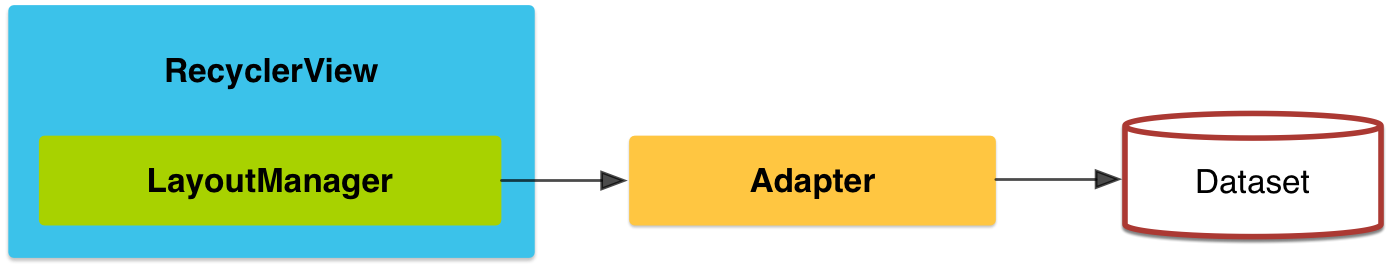
\includegraphics[width=1.0\columnwidth]{RecyclerView.png}
	\caption{Esquema RecyclerView}
	\label{fig:ejemplo}
\end{figure}

Para hacer uso de este widget es necesario definir un adaptador y un administrador de diseño. Para implementar el adaptador se extiende de la clase \textit{RecyclerView.Adapter}. En el siguiente fragmento de código se ilustra como sería la implementación del adaptador para el \textit{RecyclerView} de la lista de noticias:
\newpage
\lstinputlisting[language=java, caption={Clase NewsAdapter}, label={code:datos}]
{listings/NewsAdapter.java} %% LISTING

RecyclerView proporciona los siguientes administradores de diseño:

\begin{itemize}
\item LinearLayoutManager: muestra elementos en una lista de desplazamiento horizontal o vertical.
\item GridLayoutManager: muestra elementos en una cuadrícula.
\item StaggeredGridLayoutManager: muestra elementos en una cuadrícula escalonada.
\end{itemize}

También es posible crear administrador de diseño personalizado extendiendo de la clase \textit{RecyclerView.LayoutManager}.

En este caso se ha optado por el \textit{LinearLayout}.

\subsection{La clase ServiceActivity}
En esta clase se establece la configuración del calendario que el usuario tendrá a disposición para elegir la fecha de la reserva. Para la implemtación del calendario se ha elegido la librería \textit{MaterialCalendarView} \cite{URL::MaterialCalendarView} dado que permite, entre otras cosas, modificar la apariencia de los días, aspecto de gran utilidad a la hora de mostrar al usuario que una fecha ya está reservada.
\newline

Para ello se ha tenido que implementar la interfaz \textit{DayViewDecorator}, de esta manera a un conjunto de fechas dadas se le puede cambiar el color para que de manera intuitiva el usuario sepa que esa fecha no está disponible. 
\newline

\lstinputlisting[language=java, caption={Clase EventDecorator}, label={code:class}]
{listings/EventDecorator.java} %% LISTING

El conjunto de fechas que no están disponibles se obtiene mediante la función \textit{getReservadas} la cual hace uso de la librería \textit{Volley} \cite{URL::Volley} para hacer la petición al servidor. Se envía el identificador de la pista en la petición y en respuesta se obtiene un \textit{JSON} con las fechas reservadas (en milisegundos) para la pista dada.
\newpage
\lstinputlisting[language=java, caption={Función getReservadas}, label={code:function}]
{listings/getReservadas.java} %% LISTING

La función \textit{reserve} es muy similar a la función \textit{getReservadas} haciendo uso también de \textit{Volley} para hacer la petición. En este caso se envía el \textit{access token} para comprobar que la reserva la hace un usuario autenticado, el identificador de la pista y la fecha de reserva. En respuesta se obtiene un mensaje del servidor, que se muestra al usuario e indica si la reserva se ha podido efectuar o no. 

Al pulsar el botón reservar, se crea un \textit{dialog} \cite{URL::Dialog} que pide la confirmación del usuario antes de enviar los datos de la reserva al servidor. A continuación se ilustra como se ha implementado:

\lstinputlisting[language=java, caption={Fragmento de código del dialog}, label={code:dialog}]
{listings/dialog.java} %% LISTING

\subsection{La clase MainActivity}
En esta clase se encuentra la implementación de los eventos de la barra de acción y se realiza la gestión de los fragmentos que formarán el cuerpo de la Actividad. 

Se implementa todo lo que tiene que ver con el \textit{NavigationView} \cite{URL::NavigationView}, así como:

\begin{itemize}
\item Los eventos de mostrar y ocultar el \textit{NavigationView}.
\item Configurar la cabecera para que se muestre la información del usuario: nombre, email y foto.
\item Las eventos de los elementos del menú de navegación.
\end{itemize}

En el fragmento siguiente se muestra como se crea la transición del fragmento de la sección de noticias y como se lanza la actividad de los mapas.

\lstinputlisting[language=java, caption={Eventos de los elementos del NavigationView}, label={code:dialog}]
{listings/navigationView.java} %% LISTING

\section{Comunicación aplicación Android y el servidor}
La idea de la autenticación social es la siguiente y su unión con el servidor es 
la siguiente. Supongamos Facebook como proveedor de autenticación. En la aplicación 
móvil el usuario se autentica a través de Facebook el cual devuelve un Access Token
si resulta satisfactorio el proceso. En el caso de las aplicaciones móviles se trata 
de un token de larga duración (60 días de duración). Este token o identificador 
se actualiza una vez al día si el usuario hace una solicitud a los servidores de 
Facebook. Si el identificador llegará a caducar el usuario deberá repetir el proceso
de autenticación. Este token es enviado a nuestro servidor el cual comprueba su validez
a través de una petición a Facebook, en caso de que sea válido el usuario es considerado
autenticado en nuestro servidor y se utilizará dicho token para poder acceder a los 
distintos servicios disponibles.